\chapter{Evaluation und Validation}
\label{ch:Eval}

Die  Softwarearchitektur wurde während der Realisierung mit einem kleineren Datensatz mit 100000 Ratings getestet. Nach Beendigung der Realisierung der Softwararchitektur, wurde festgestellt, das mit den gegebenen Ressourcen, keine Berechnung der Top $N$ Nachbarn mit 25 Millionen Ratings möglich ist.
Nach Absprache mit dem Betreuer Tahir Majeed, wurden die Top N Nachbarn mit 1 Million, 2 Millionen, 5 Millionen und 7 Millionen Ratings berechnet.

\begin{figure}[htb]
	\centering
	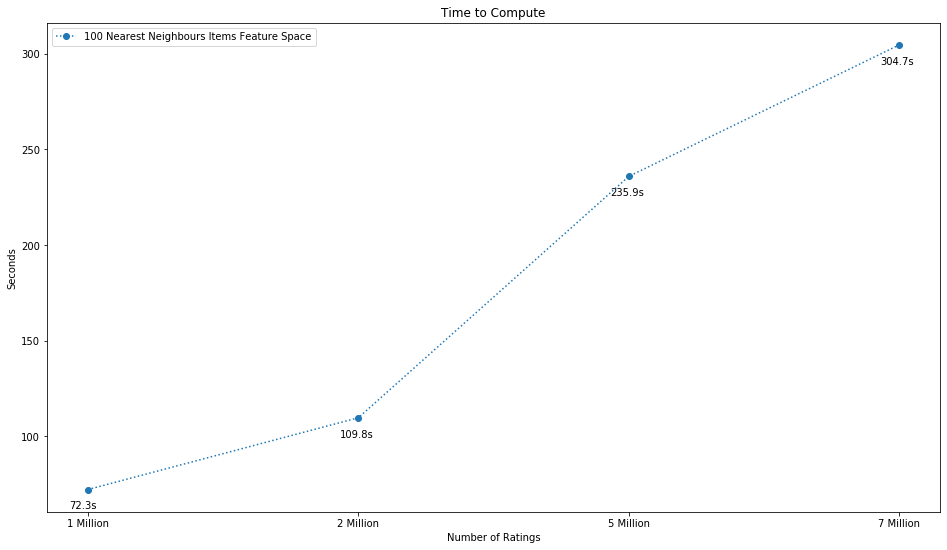
\includegraphics[keepaspectratio,width=\linewidth]{img/Time to Compute Items Featurespace.png}
	\caption{Rechenzeit Top 100 Item Nachbarn Featurespace}
	\label{fig:Rechenzeit Itemnachbarn Featurespace}
\end{figure}

In Abbildung \ref{fig:Rechenzeit Itemnachbarn Featurespace} sieht man, dass die Rechenzeit von 304 Sekunden (ungefähr 5 Minuten) im Featurespace auch mit 7 Millionen Ratings relativ kurz ist. Auch die Berechnung der Top 100 User Nachbaren ist mit 596 Sekunden (ungefähr 10 Minuten), wie in Abbildung \ref{fig:Rechenzeit Usernachbarn Featurespace} ersichtlich, relativ schnell. 

\begin{figure}[h!tb]
	\centering
	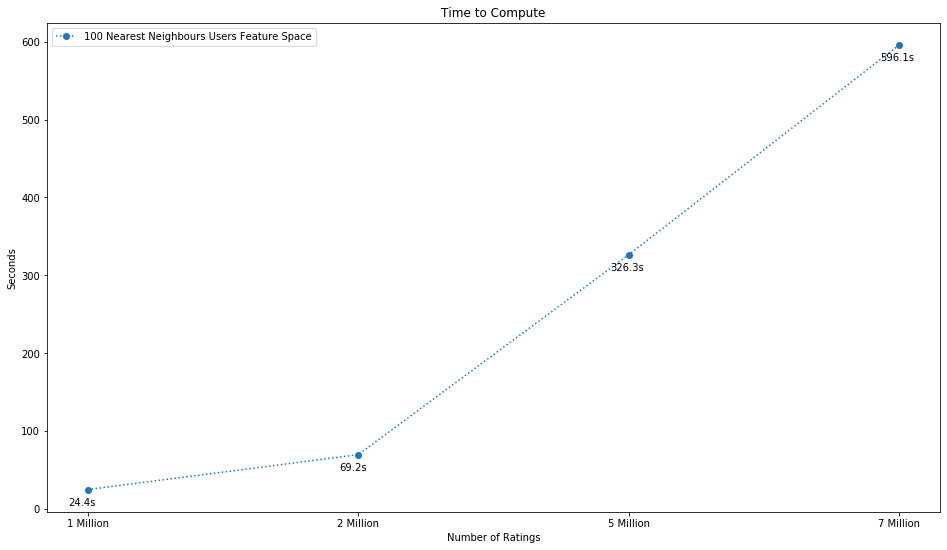
\includegraphics[keepaspectratio,width=\linewidth]{img/Time to Compute User Featurespace.png} 
	\caption{Rechenzeit Top 100 User Nachbarn Featurespace}
	\label{fig:Rechenzeit Usernachbarn Featurespace}
\end{figure}
Wie in Abbildung \ref{fig:Rechenzeit Featurespace} zu sehen ist, sieht man aber schon einen Unterschied zwischen der Berechnung der User und Item Nachbarn.
\begin{figure}[h!tb]
	\centering
	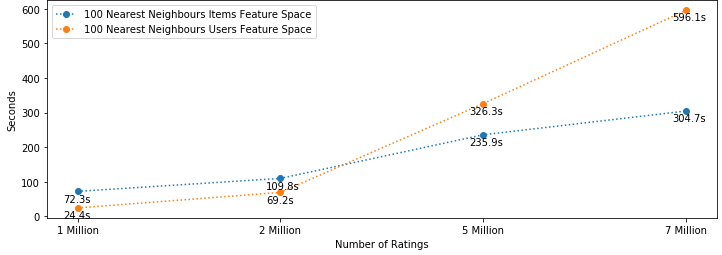
\includegraphics[keepaspectratio,width=\linewidth]{img/Time to Compute Featurespace.png} 
	\caption{Rechenzeit Top 100 Nachbarn Featurespace}
	\label{fig:Rechenzeit Featurespace}
\end{figure}

%TODO Einfügen von Abbildung und Referenz
Werden aber die Top 100 Nachbarn im PCA Space gesucht explodiert die Rechenzeit enorm. Wieder mit 1 Million Ratings beginnend, starten wir bei der Berechnung der 100 Top Item Nachbarn im PCA Space bei einer Rechenzeit von 675 Sekunden (siehe Abbildung ). Dies überschreitet bereits mit nur 1 Million Ratings die Rechenzeit der Top 100 Item und User Nachbarn im Featurespace. Betrachten wir nun die Rechenzeit für 2 Millionen Ratings aus Abbildung X, sehen wir, dass die Rechenzeit mit 4112 Sekunden (circa 69 Minuten) bereits jetzt um das \textbf{sechsfache} gestiegen ist.

\section{Resultate}


Waren die eingesetzten Methoden zweckmässig?
- Sind die Ergebnisse aussagekräftig und zuverlässig?
- Sind die Ergebnisse auf andere Gebiete übertragbar?
- In welchem Verhältnis stehen die Ergebnisse zur übrigen Forschung? Decken sie sich oder
widersprechen sie ihr?
- Welche Bedeutung haben die Ergebnisse für die Praxis?
- Welche Bedeutung haben die Ergebnisse für weitere Forschungen?

\section{Vergleich mit Anforderungen}
\label{sec:VergleichAnforderungen}
% TODO Vergleich mit Anforderungen Soll<->Ist

\section{Technische Aspekte}
% TODO Evaluation der verwendeten Hilfsmittel

\section{Vorgehen}
% TODO Evaluation der verwendeten Arbeitsprozesse
